\section{Übung - Modellierung}
\label{sec:uebung_03}
Entwickeln Sie auf Basis des folgenden Schemas einen Entwurf für ein Data Warehouse. Verwenden Sie dazu den Oracle Data Modeler und erzeugen Sie im ersten Schritt ein logisches Modell um anschließend daraus ein relationales Star- und ein relationales Snowflake-Modell entwickeln zu lassen. Lassen Sie sich die DDL-Statements zur Erzeugung der modellierten Tabellen ausgeben.

\begin{figure}[H]
  \centering
  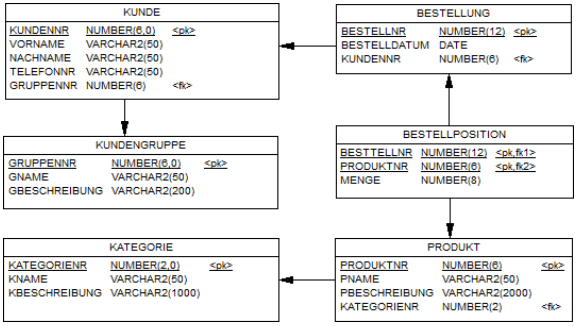
\includegraphics[width=0.85\textwidth]{img//uebung_03_-_schema.png}
  \label{img:uebung_03_-_schema}
  \caption{Schema}
\end{figure} 

Verwenden Sie folgende Leitfragen zur Identifizierung der Granularität und Dimensionen:
\begin{itemize}
  \item Wie viele Produkte wurden 2014 an den Kunden mit der Kundennummer 123 verkauft?
  \item In welcher Kundengruppe wurden im Januar 2015 die meisten Produkte abgesetzt?
  \item Wie oft wurde das Produkt „Ebook-Reader ABC“ am 03.01.2013 verkauft.
  \item Wie viele Produkte der Kategorie „Online-Medien“ wurden am 03.03.2013 um 00:11 verkauft?
  \item In welcher Stunde wurden am 01.01.2016 die meisten Produkte der Produktkategorie **Printmedien** abgesetzt?
  \item Wie viele Produkte der Produktkategorie „Printmedien“ wurden vormittags am 04.02.2013 abgesetzt?
\end{itemize}